\documentclass[12pt,a4paper,openright,twoside]{report}
\usepackage[italian]{babel}
\usepackage[latin1]{inputenc}
\usepackage{graphicx}
\usepackage{amssymb}
\usepackage{amsmath}
\usepackage{latexsym}
\usepackage{amsthm}
\oddsidemargin=30pt \evensidemargin=20pt
\hyphenation{sil-la-ba-zio-ne pa-ren-te-si}
\usepackage{tgtermes}
\usepackage{tikz}
\usepackage{pgfplots}
\pgfplotsset{compat=1.18}
\makeatletter
% Capitoli numerati
\def\@makechapterhead#1{%
	\vspace*{-80pt}% spazio dall'alto pagina
	{\parindent \z@ \raggedright \normalfont
		\Huge\bfseries
		\thechapter\quad #1\par\nobreak
		\vskip 20pt
}}

% Capitoli NON numerati
\def\@makeschapterhead#1{%
	\vspace*{-80pt}% spazio dall'alto pagina
	{\parindent \z@ \raggedright
		\normalfont
		\Huge\bfseries
		#1\par\nobreak
		\vskip 20pt
}}

\makeatother
\begin{document}
\begin{titlepage}
	\begin{center}
		
		% Nome ufficiale dell'Ateneo: NON modificare.
		{{\Large{\textsc{Alma Mater Studiorum $\cdot$ Universit\`a di
						Bologna}}}} \rule[0.1cm]{15.8cm}{0.1mm}
		\rule[0.5cm]{15.8cm}{0.6mm}
		
		% ------------------------------------------------------------------
		% DIPARTIMENTO / CORSO DI LAUREA
		% ------------------------------------------------------------------
		% Selezionare il corso di Laurea di riferimento, cancellando le opzioni non necessarie.
		%
		{\small{\bf TODO Dipartimento di Informatica --- Scienza e Ingegneria\\
				Corso di Laurea Triennale in Ingegneria e Scienze informatiche}}
	\end{center}
	
	\vspace{15mm}
	\begin{center}
		% ------------------------------------------------------------------
		% TITOLO DELLA TESI
		% ------------------------------------------------------------------
		% Sostituire "TITOLO DELLA TESI" con il titolo completo della propria tesi.
		% Suggerimenti:
		% - Usare MAIUSCOLO per il titolo principale, se richiesto dalle linee guida.
		% - Evitare abbreviazioni non standard.
		{\LARGE{\bf TODO}}\\
		\vspace{3mm}
		
		\vspace{19mm}
		% ------------------------------------------------------------------
		% SETTORE SCIENTIFICO DI RIFERIMENTO (OPZIONALE)
		% ------------------------------------------------------------------
		% Questa riga è opzionale. Puoi:
		% - Sostituire "Settore Scientifico di Riferimento" con il nome dell'insegnamento
		%   o ambito disciplinare da cui nasce la tesi (es. "Machine Learning", "Calcolo Numerico").
		% - Oppure, se non richiesto dal tuo Corso di Laurea, puoi COMMENTARE
		%   l'intera riga anteponendo un % all'inizio.
		{\large{\bf TODO}}
	\end{center}
	
	\vspace{30mm}
	\par
	\noindent
	\begin{minipage}[t]{0.50\textwidth}
		% ------------------------------------------------------------------
		% RELATORE
		% ------------------------------------------------------------------
		% Sostituire:
		% - "Chiar.ma Prof." con il titolo corretto del relatore:
		%    * "Chiar.mo Prof." / "Chiar.ma Prof.ssa"
		%    * oppure "Prof." / "Prof.ssa" / "Dott." / "Dott.ssa"
		%   a seconda di quanto concordato con il/la relatore/relatrice.
		% - "NOME RELATORE" con Nome e Cognome del relatore.
		{\large{\bf Relatore:\\
				Chiar.ma Prof.\\
				TODO}} \\[5mm]
		
		% ------------------------------------------------------------------
		% CORRELATORE (FACOLTATIVO)
		% ------------------------------------------------------------------
		% Se HAI un correlatore:
		%   - Sostituisci "Chiar.mo Prof." con il titolo accademico corretto.
		%   - Sostituisci "NOME CORRELATORE" con Nome e Cognome del correlatore.
		%
		% Se NON hai un correlatore:
		%   - Commenta il blocco qui sotto anteponendo % a ciascuna riga,
		%     oppure cancellalo.
		\large{\bf Correlatore: \\
			Chiar.mo Prof. \\
			TODO}
	\end{minipage}
	\hfill
	\begin{minipage}[t]{0.47\textwidth}\raggedleft
		% ------------------------------------------------------------------
		% NOME DELLAUREANDO / LAUREANDA
		% ------------------------------------------------------------------
		% Sostituire "NOME LAUREANDO" con:
		%   Nome Cognome
		% esattamente come compare nei documenti ufficiali.
		{\large{\bf Presentata da:\\
			TODO}}
	\end{minipage}
	
	\vspace{10mm}
	\begin{center}
		% ------------------------------------------------------------------
		% APPELLO, DATA E ANNO ACCADEMICO
		% ------------------------------------------------------------------
		% "NUMERO Appello":
		%   - Sostituire con il numero dell'appello di laurea (es. "I Appello", "II Appello")
		%     secondo le indicazioni della Segreteria/CdS.
		%
		% "Sessione MESE ANNO":
		%   - Sostituire con la data ufficiale della seduta di laurea
		%
		% "Anno Accademico 20xx/20xx":
		%   - Sostituire con l'Anno Accademico corretto (es. "Anno Accademico 2025/2026").
		{\large{\bf Sessione MESE ANNO \\}}
		{\large{\bf Anno Accademico 20TODO/20xx\\}}
	\end{center}
\end{titlepage}
\clearpage{\pagestyle{empty}\cleardoublepage}
\cleardoublepage
\tableofcontents
\cleardoublepage
\listoffigures
\cleardoublepage
\listoftables
\clearpage{\pagestyle{empty}\cleardoublepage}

\chapter*{Sommario}
\setcounter{page}{9}
\thispagestyle{plain}
	TODO
	IoT (Internet of Things) è l'acronimo utilizzato per indicare la sfera tecnologica che ha alla base l'utilizzo di oggetti intelligenti. 
	Per oggetti intelligenti si intendono quei dispositivi, macchine o attrezzature che si possono connettere a internet per trasmettere, ricevere dati o elaborarli.
	All'interno di questa sfera, uno dei metodi di comunicazione più utilizzati è quello basato su un modello Publish/Subscribe che consente lo scambio di dati tra dispositivi della rete senza la necessità di connessioni dirette tra loro.
	Per funzionare si utilizza il protocollo MQTT, uno dei protocolli più diffusi per lo scambio di messaggi, il quale si basa su una struttura con 3 tipologie di dispositivi connessi: Publisher, Subscriber e Broker.
	I Publisher una volta ottenuti dei dati tramite sensori di vario genere, li pubblica, rendendoli disponibili nella rete. I dati per spostarsi all'interno della rete utilizzano i broker cioè vari punti/server di connessione, i quali permettono il passaggio di dati per poi infine arrivare ai Subscribers per la lettura e l'elaborazione.
	Questa tesi riprende il lavoro effettuato da un collega nell'anno 21-22 approfondendo e sviluppando i casi di test con particolare attenzione a quelle che sono le caratteristiche che 
	possono portare criticità al calcolo della soluzione ottima di percorso per il flusso dei dati.
	La tesi del collega si basa sull'idea di costruire un sistema distribuito sfruttando le proprietà matematiche del rilassamento Lagrangiano, dove ogni nodo conosce solamente i propri vicini.
\chapter{Introduzione}     
\vspace{-0.5cm}        
\section{Iot (Internet of Things)}    
\vspace{-0.3cm}          
Il termine Iot nasce come acronimo per indicare quella sfera tecnologica moderna che si basa sull'utilizzo di dispositivi "intelligenti". Quest'ultima ha avuto particolare rilevanza nell'ultimo periodo storico, andando a rivoluzionare il modo in cui si raccolgono e si processano le informazioni sia in ambito domestico sia industriale. \smallskip \\
Un dispositivo definito intelligente o più comunemente chiamato "smart" è un dispositivo in grado di connettersi alla rete per poter svolgere diverse funzioni in cui tra le più importanti è presente lo scambio di informazioni. \smallskip \\
In questa tesi ci si sofferma particolarmente sui "sensori", dispositivi chiave per lo scambio di messaggi in una rete IoT.
Un sensore è un dispositivo che rileva un cambiamento nel mondo fisico, lo traduce in un segnale digitale e poi lo diffonde ad altri dispositivi, i quali lo utilizzeranno per prendere decisioni. \smallskip \\
Una possibile criticità risiede proprio in questa parte del funzionamento, se una decisione deve essere presa con tempestività, anche la rete di trasmissione dovrà essere veloce e efficiente.
\vspace{-0.5cm}
\section{Publish and Subscribe}
\vspace{-0.3cm}   
Tra le metodologie più famose di trasmissione di messaggi, quella che si intende approfondire è il Publish and Subscribe, un paradigma particolarmente adatto all'IoT, nato come sostituzione del classico Client-Server. In questo schema i dispositivi si dividono in Publisher e Subscriber collegati tra loro tramite dei nodi/server di trasmissione definiti Broker. \smallskip \\
In questo modello ognuno ha il suo ruolo: i Publisher devono diffondere nella rete le informazioni in loro possesso, i Broker devono ritrasmettere queste informazioni senza permettere danneggiamenti o perdita delle stesse e i Subscriber sono i ricevitori o i richiedenti.
Per quanto riguarda il meccanismo alla base è molto semplice: il Publisher invia messaggi etichettati con un topic, il Broker li riceve e li inoltra solamente ai Subscriber iscritti a quel topic. \smallskip \\ Questo approccio permette un disaccoppiamento tra nodo di partenza e di arrivo, in quanto le due parti non si conoscono direttamente e non devono per forza essere attive contemporaneamente per garantire il successo della comunicazione. \smallskip \\
Il protocollo standard per l'implementazione di questo modello è l'MQTT, progettato per essere leggero e robusto anche su reti instabili ma che presenta alla base una criticità importante: essendo il Broker il nodo centrale di comunicazione, la sua irraggiungibilità diventa rischio di interruzione per l'intera rete. Per ovviare al problema, si è optato per la creazione di infrastrutture con più Broker configurati per lavorare e apparire come uno solo, in modo che nel caso di fallimento di un server, i rimanenti possano continuare il lavoro.\smallskip \\ Facendo riferimento al paragrafo precedente si può associare il ruolo di Publisher ai sensori e il ruolo di Subscriber a tutti quei dispositivi che necessitano del valore rilevato.
\begin{figure}[h]
	\centering
	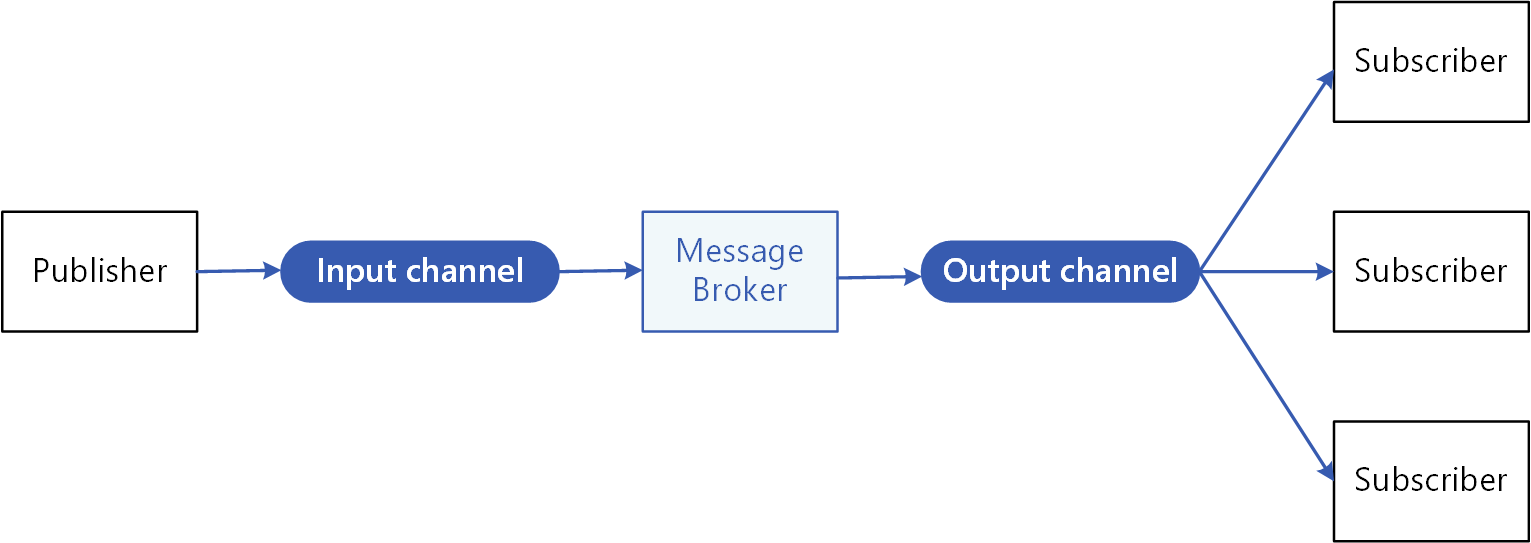
\includegraphics[width=1\linewidth]{publish-subscribe}
	\caption[Immagine di funzionamento di una rete Publish and Subscribe]{Immagine di funzionamento di una rete Publish and Subscribe}
	\label{fig:publish-subscribe}
\end{figure}
\section{La difficoltà del percorso ottimo}
In un sistema moderno, trovare il percorso ottimo per la trasmissione dei dati è cruciale, infatti una scelta non ottimizzata potrebbe ritardare o addirittura impedire la ricezione delle informazioni, compromettendo il funzionamento dei dispositivi che dipendono da esse. Per questo motivo è necessario individuare il metodo più efficiente per rappresentare la rete e per calcolare il percorso ottimale.
\subsection{Grafo}
Uno dei metodi migliori per poter descrivere una rete di dispositivi connessi è tramite un grafo. Usando questa struttura, i dispositivi vengono rappresentati tramite dei nodi e i collegamenti tramite degli archi. \begin{figure}[h]
	\centering
	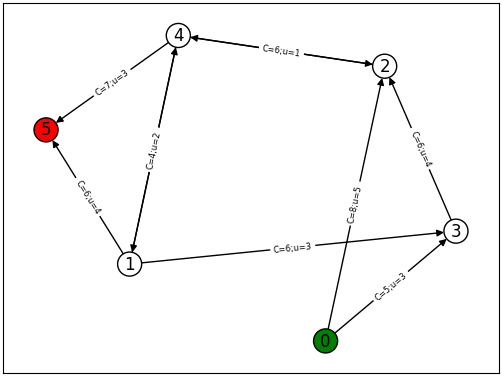
\includegraphics[width=0.7\linewidth]{Grafo}
	\caption[Immagine di un grafo con costi e capacità degli archi]{Immagine di un grafo con costi e capacità degli archi}
	\label{fig:grafo}
\end{figure}\newpage 
\noindent L'uso di un grafo risulta una scelta efficiente perché, per reti semplici, consente di mostrare in modo naturale sia i componenti della rete sia le relazioni tra essi e grazie alla sua flessibilità permette inoltre di aggiungere varie proprietà agli elementi rappresentati, rendendo possibile modellare scenari complessi con facilità.
\textbf{TODO Capire se mi conviene parlare della centralizzazione e del 2p2 dato che lavoro più in un ambito non decentralizzato nel mio caso}
\subsection{Centralizzazione}
Un altro aspetto fondamentale del problema riguarda la centralizzazione dell'elaborazione della rete.
In un caso reale, calcolare qual è il percorso ottimo necessita di una notevole potenza di calcolo e, soprattutto, bisogna che ci sia la garanzia di possedere informazioni complete sulla composizione della rete.
Da qui nasce l'idea di non affidarsi più esclusivamente ad un server centrale ma di distribuire il calcolo su tutti i dispositivi della rete rendendola autonoma sia nella ricerca del percorso ottimo sia nella gestione dei guasti in caso di malfunzionamento di un canale.
\subsubsection{Peer-To-Peer}
Ciò è reso possibile sfruttando un protocollo Peer-to-Peer, ovvero un protocollo che tratta i dispositivi in comunicazione sia come Client sia come Server, permettendogli dunque di scambiarsi richieste di risorse o servizi senza dover passare da terzi.
\textbf{TODO origini del p2p, strutturati e non strutturati, problemi legati al p2p}.

\section{Problema di ottimizzazione}
Il problema descritto è così definito come un problema di ottimizzazione, problema che richiede di trovare la migliore soluzione possibile fra tutte le soluzioni ammissibili, massimizzando o minimizzando una funzione definita obiettivo e rispettando i vincoli imposti. \smallskip \\
Questo tipo di problema è descrivibile utilizzando un modello matematico:
\begin{equation}
	min/max\ \sum_i c_ix_i
\end{equation}
s.t 
\begin{equation}
	Ax \geq  b
\end{equation}
\vspace{-0.6cm}
\begin{equation}
	Bx \geq  d 
\end{equation}
\vspace{-0.6cm}
\begin{equation}
	x \in \{0, 1\}
\end{equation}
Con $c$ il vettore dei costi, $x$ la variabile decisionale, $A$ e $B$ le matrici dei coefficienti del problema, $b$ e $d$ i vettori delle costanti per i vincoli.\smallskip \\
Molto spesso quando si tratta di problemi di questo tipo, si possono riscontrare delle difficoltà nella risoluzione, per questo viene adottata la tecnica del rilassamento dei vincoli che consente di semplificare il calcolo ottenendo un limite inferiore per la soluzione del problema originale.
\subsection{Rilassamento Continuo}
Il rilassamento più intuitivo è quello continuo, dove se il problema presenta la variabile decisionale come intera, è possibile costruire un problema di ottimizzazione equivalente, abbandonando il vincolo di interezza della variabile e permettendole di assumere un qualsiasi valore reale all'interno di un intervallo continuo derivato dal vincolo originale. \smallskip \\
Questo approccio trasforma il problema intero in un problema di programmazione lineare continua, per il quale esistono algoritmi efficienti. Lo spazio delle soluzioni ammissibili, tuttavia, è più ampio e il valore ottimo del problema rilassato potrebbe non essere sempre applicabile al problema originale.
\begin{equation}
 x \in \{0, 1\}  \rightarrow 0 \leq	x \leq 1
\end{equation}
\subsection{Rilassamento Lagrangiano}
Un rilassamento particolarmente utile è quello lagrangiano, che permette di rilassare i vincoli computazionalmente dispendiosi aggiungendoli alla funzione obiettivo e associando a ognuno di essi un moltiplicatore di Lagrange. Quest'ultimo funge da penalità: più ci si allontana dal rispetto del vincolo, maggiore sarà il peggioramento del valore della funzione obiettivo, allontanandolo dall'ottimo. Il risultato è una nuova funzione obiettivo, detta lagrangiana, che dipende sia dalle variabili originali del problema sia dai moltiplicatori di Lagrange, e la cui risoluzione fornirà i valori ottimi di entrambi.
\subsubsection{Spiegazione matematica}
Consideriamo un problema di minimizzazione \textbf{P}:
\begin{equation}
	z(P)=min\ cx 
\end{equation}
s.t 
\begin{equation}
	Ax \geq  b
\end{equation}
\begin{equation}
	x \in \{0, 1\}
\end{equation}
Con $c$ il vettore dei costi, x la variabile decisionale, A la matrice dei coefficienti del problema, b il vettore delle costanti per il vincolo. \smallskip \\
Con il rilassamento lagrangiano si rilassa il vincolo $Ax \geq b$ aggiungendo una penalità $\lambda$ non negativa e inserendolo all'interno della funzione obiettivo.
\begin{equation}
	z(P)=min\ cx,\ Ax-b \geq 0
\end{equation}
$$\downarrow$$
\begin{equation}
	L(\lambda)=min\ cx-\lambda(Ax-b)
\end{equation}
s.t
\begin{equation}
	x \in \{0, 1\}
\end{equation}
Il motivo del segno $-$ è dovuto al fatto che il vincolo è soddisfatto quando assume un valore maggiore o uguale a 0, quindi dato che $\lambda$ è definita non negativa, se il vincolo non viene soddisfatto come nel caso in cui sia negativo, sottrarlo dalla funzione obiettivo ne aumenta il valore, allontanandolo dal minimo ricercato.\vspace{0.15cm}  \\  Il valore ottimale del problema originale $z(P)$ sarà maggiore o al massimo uguale al valore ottimale del problema rilassato $L(\lambda)$. 
\begin{align}
	z(P)\geq L(\lambda),\ \ \ \ \forall \lambda \geq 0
\end{align}
Questo perché non avendo l'obbligo di rispettare il vincolo, che è stato rilassato, lo spazio delle soluzioni ammissibili è più ampio e quindi si possono trovare soluzioni che il problema originale non può considerare corrette, le quali, avendo meno costrizioni, avranno un valore più basso o al massimo uguale alla soluzione dell'originale. 
\begin{enumerate}
	\item Si prende una $x^*$ che è soluzione ottima di $z(P)$ quindi è ammissibile e il vincolo è rispettato.
	\item Per $\lambda \geq 0$ e $Ax^* - b\geq 0$ si ha: \begin{equation}
		cx^* \geq cx^* - \lambda(ax^*-b)
	\end{equation}
	\item $x^*$ è anche soluzione ammissibile per il problema rilassato quindi esiste sicuramente una soluzione di $L(\lambda)$ che sarà o minore o uguale al valore di $x^*$:
	\begin{equation}
		L(\lambda)=\min(cx-\lambda(Ax-b))\leq cx^*-\lambda(Ax^*-b)
	\end{equation}\vspace{-0.75cm}
	\item Unendo le diseguaglianze: \begin{equation}
		z(P)=cx^* \geq cx^* - \lambda(ax^*-b)\geq L(\lambda) \rightarrow z(P)\geq L(\lambda)
	\end{equation}
	
\end{enumerate}
%
%In ogni caso dove il vincolo è rispettato, il valore di $\lambda(Ax-b)$ è non negativo:
%\begin{equation}
%	z(P)=cx \geq cx-\lambda(Ax-b)=L(\lambda)
%\end{equation}
%In caso invece non fosse rispettato i due risultati non sarebbero confrontabili in quanto non esisterebbe una soluzione ammissibile per l'originale. \smallskip \\
Grazie a questa proprietà, si può pensare di massimizzare la funzione lagrangiana per ottenere il migliore limite inferiore possibile per il problema originale e si può descrivere con la formula del duale lagrangiano:
\begin{equation}
	z(D_L)=\max_{\lambda\geq0}\ [L(\lambda)]
\end{equation}
Una delle tecniche che può essere usata per la ricerca della soluzione del duale lagrangiano è il metodo del sottogradiente.
\subsubsection{Metodo del sottogradiente}
Il metodo del sottogradiente è un metodo iterativo usato per massimizzare una funzione concava, come quella lagrangiana, con lo scopo di ottenere il migliore limite inferiore per il problema originale. Nello specifico, si può utilizzare per calcolare i moltiplicatori di Lagrange associati ai vincoli rilassati che forniscono il risultato $L(\lambda)$ più alto. \smallskip \\
La funzione lagrangiana non è perfettamente una curva liscia ma è composta di segmenti, ciascuno corrispondente a una soluzione ottima $\bar{x}$ per il $\lambda$ specificato.
\begin{figure}[h]
	\centering
	\begin{tikzpicture}
		\begin{axis}[
			axis lines=left,
			xlabel={$\lambda$},
			ylabel={$L(\lambda)$},
			xmin=0, xmax=5,
			ymin=0, ymax=4.5,
			xtick=\empty,
			ytick=\empty,
			width=8cm,
			height=6cm,
			clip=false
			]
			\addplot[blue, very thick, smooth, domain=0.5:4.7, samples=100]
			{-0.3667*(x-3)^2 + 3.5};
			\addplot[red, thick, smooth] coordinates {(0.2,0.86) (1.8,3.21)};  
			\addplot[red, thick, smooth] coordinates {(1.2,2.55) (2.8,3.72)};  
			\addplot[red, thick, smooth] coordinates {(2.2,3.5) (3.8,3.5)};    
			\addplot[red, thick, smooth] coordinates {(3.2,3.72) (4.8,2.55)};   
		\end{axis}
	\end{tikzpicture}
	\caption{Immagine di una funzione lagrangiana con inviluppo}
	\label{fig:lagrangiana_inviluppo}
\end{figure}
\newpage
\noindent 
Data una lambda, si ottiene una $\bar{x}$ tale che:
\begin{equation}
	L(\bar{\lambda})=\min (cx-\bar{\lambda}(Ax-b))=c\bar{x}-\bar{\lambda}(A\bar{x}-b)
\end{equation}
\begin{figure}[h]
	\centering
	\begin{tikzpicture}
		\begin{axis}[
			axis lines=left,
			xlabel={$\lambda$},
			ylabel={$L(\lambda)$},
			xmin=0, xmax=5,
			ymin=0, ymax=4.5,
			xtick=\empty,
			ytick=\empty,
			width=8cm,
			height=6cm,
			clip=false
			]
			\addplot[blue, very thick, smooth, domain=0.5:4.7, samples=100]
			{-0.3667*(x-3)^2 + 3.5};
			\addplot[black, densely dotted, thin] coordinates {(1.4,0) (1.4,2.561)};
			\addplot[black, densely dotted, thin] coordinates {(0,2.561) (1.4,2.561)};
			\node at (axis cs:1.4, 2.561) [anchor=south, yshift=4pt] {$L(\bar{\lambda})$};
			\node at (axis cs:1.4, 0) [anchor=north, yshift=-4pt] {$\bar{\lambda}$};
		\end{axis}
	\end{tikzpicture}
	\caption{Valore di $L(\bar{\lambda})$ corrispondente a una $\bar{\lambda}$ scelta}
	\label{fig:Determinisco di L scelta una lambda}
\end{figure} \\
Riprendendo la soluzione $\bar{x}$ derivata dalla $\bar{\lambda}$ data possiamo ridefinire $L(\lambda)$ cioè la soluzione in una qualsiasi altra lambda generica come o migliore o uguale della soluzione trovata ora:
\begin{equation}
	L(\lambda)=\min (cx-\lambda(Ax-b))\leq c\bar{x}-\lambda(A\bar{x}-b)
\end{equation}
Questo perché se si prende un'altra $\lambda$, noi confrontiamo nel lato sinistro la $x$ ottimale per quel $\lambda$ con nel lato destro la $\bar{x}$ non per forza ottimale con lo stesso $\lambda$.
In pratica se teniamo la stessa $\lambda$ e confrontiamo giustamente la sua x ottima allora sarà migliore di un'altra x a caso nel nostro caso $\bar{x}$ con stessa lambda. (la cosa ovviamente sarebbe stata diversa con lambda diverse cioè se confrontata x ottima per $\lambda$ con $\bar{x}$ ottima per $\bar{\lambda}$ non si sa quale L darebbe di meno.)
Sottraendo ora l'equazione (1.17) dalla (1.18) otteniamo:
\begin{equation}
	L(\lambda)-L(\bar{\lambda})\leq c\bar{x}-\lambda(A\bar{x}-b)-(c\bar{x}-\bar{\lambda}(A\bar{x}-b))
\end{equation}
$$\downarrow$$
\begin{equation}
	L(\lambda)-L(\bar{\lambda})\leq -\lambda(A\bar{x}-b)+\bar{\lambda}(A\bar{x}-b)
\end{equation}
$$\downarrow$$
\begin{equation}
	L(\lambda)-L(\bar{\lambda})\leq (A\bar{x}-b)(-\lambda+\bar{\lambda})
\end{equation}
$$\downarrow$$
\begin{equation}
	L(\lambda)\leq L(\bar{\lambda})+(A\bar{x}-b)(-\lambda+\bar{\lambda})
\end{equation}
Definiamo $s=-(A\bar{x}-b)$
Così poi diventa $L(\lambda)-L(\bar{\lambda})<=s(\lambda-\bar{\lambda})$
Noi vogliamo che L lambda sia > di L \bar{lambda} quindi che la loro differenza sia > 0
Per ottenere questo risultato è importante che dato che L(\lambda) <=  L(\bar{lambda})+s(\lambda-\bar{lambda}) la parte a dx sia positiva:
s(\lambda-\bar{lambda})>0
Quindi lo spostamento \lambda-\bar{lambda} deve avere lo stesso verso del subgradiente s ed è per questo che si sceglie \lambda = \bar{lambda}+0s così lo spostamento segue il verso di lambda
infatti \lambda - \bar{lambda}=0s
s(\lambda-\bar{lambda})=s(0s)=0s^2 che è sicuramente >0 per uno step positivo e s!=0 quindi ci stiamo muovendo nella stessa direzione che tende ad aumentare L


Quindi abbiamo un upper bound sulla differenza quindi in pratica non possiamo avere una differenza più alta del valore del subgradiente per la differenza dei lambda.
E noi vogliamo massimizzare $L(\lambda)$ quindi vogliamo che $L(\lambda)-L(\bar{\lambda})$ risulti $>$ di 0 cioè il nuovo L sia maggiore del precedente.
Per garantire ciò vogliamo che s per la differenza dei lambda sia positiva perché se fosse negativa $L(\bar{lambda})$ + un valore negativo verrebbe sicuramente più piccola mentre se è positivo aumenta.
Per fare in modo che sia positiva allora bisogna che s sia di base presa come positiva e la nuova lambda sia > della vecchia
Se mi muovo nella direzione del subgradiente questo funziona.

In generale per una funzione f un vettore s è subgradiente in un punto y se rispetta la seguente formual f(x)<=f(y)+s(x-y).
Dato che vogliamo massimizzare L(lambda) e portarlo a un miglioramento allora l'unica sperianza che abbiamo è sommare a L(\bar{lambda}) un valore positivo.

\section{Ambiente di sviluppo}

\chapter{nella parte del problema spiegare che ci sono costi e capacità}



%Ora vediamo un elenco numerato:         %crea un elenco numerato
%\begin{enumerate}
%\item primo oggetto
%\item secondo oggetto
%\item terzo oggetto
%\item quarto oggetto
%\end{enumerate}
%
%\begin{figure}[h]                       %crea l'ambiente figura; [h] sta
%                                        %   per here, cioè la figura va qui
%\begin{center}                          %centra nel mezzo della pagina
%                                        %   la figura
%%\includegraphics[width=5cm]{figura.eps}%inserisce una figura larga 5cm
%                                        %se si vuole usare va scommentata
%%
%%%%%%%%%%%%%%%%%%%%%%%%%%%%%%%%%%%%%%%%%%inserisce la legenda ed etichetta
%                                        %   la figura con \label{fig:prima}
%\caption[legenda elenco figure]{legenda sotto la figura}\label{fig:prima}
%\end{center}
%\end{figure}
%
%\section{Seconda Sezione}
%Ora vediamo un elenco puntato:
%\begin{itemize}                         %crea un elenco puntato
%\item primo oggetto
%\item secondo oggetto
%\end{itemize}
%
%\section{Altra Sezione}
%Vediamo un elenco descrittivo:
%\begin{description}                     %crea un elenco descrittivo
%  \item[OGGETTO1] prima descrizione;
%  \item[OGGETTO2] seconda descrizione;
%  \item[OGGETTO3] terza descrizione.
%\end{description}
%%%%%%%%%%%%%%%%%%%%%%%%%%%%%%%%%%%%%%%%%%crea una sottosezione
%\subsection{Altra SottoSezione}
%%%%%%%%%%%%%%%%%%%%%%%%%%%%%%%%%%%%%%%%%%crea una sottosottosezione
%\subsubsection{SottoSottoSezione}Questa sottosottosezione non viene
%numerata, ma \`e solo scritta in grassetto.
%\section{Altra Sezione}                 %crea una sottosezione
%Vediamo la creazione di una tabella; la tabella \ref{tab:uno}
%(richiamo il nome della tabella utilizzando la label che ho messo sotto):
%la facciamo di tre righe e tre colonne, la prima colonna
%``incolonnata'' a destra (r) e le altre centrate (c):\\
%\begin{table}[h]                        %ambiente tabella
%                                        %(serve per avere la legenda)
%\begin{center}                          %centra nella pagina la tabella
%\begin{tabular}{r|c|c}                  %tre colonne con righe verticali
%                                        %   prodotte con |
%\hline \hline                           %inserisce due righe orizzontali
%$(1,1)$ & $(1,2)$ & $(1,3)$\\           %& separa le colonne e con
%\hline                                  %inserisce una riga orizzontale
%$(2,1)$ & $(2,2)$ & $(2,3)$\\           %  \\ va a capo
%\hline                                  %inserisce una riga orizzontale
%$(3,1)$ & $(3,2)$ & $(3,3)$\\
%\hline \hline                           %inserisce due righe orizzontali
%\end{tabular}
%\caption[legenda elenco tabelle]{legenda tabella}\label{tab:uno}
%\end{center}
%\end{table}
%\section{Altra Sezione}\label{sec:prova}%posso mettere le label anche
%                                        %   alle section
%\subsection{Listati dei programmi}
%\subsubsection{Primo Listato}
%\begin{verbatim}
%        In questo ambiente     posso scrivere      come voglio,
%lasciare gli spazi che voglio e non % commentare quando voglio
%e ci sarà scritto tutto.
%Quando lo uso è meglio che disattivi il Wrap del WinEdt
%\end{verbatim}
%%%%%%%%%%%%%%%%%%%%%%%%%%%%%%%%%%%%%%%%%%non numera l'ultima pagina sinistra
%\clearpage{\pagestyle{empty}\cleardoublepage}
%%%%%%%%%%%%%%%%%%%%%%%%%%%%%%%%%%%%%%%%%%per fare le conclusioni
%\chapter*{Conclusioni}
%%%%%%%%%%%%%%%%%%%%%%%%%%%%%%%%%%%%%%%%%%imposta l'intestazione di pagina
%%%%%%%%%%%%%%%%%%%%%%%%%%%%%%%%%%%%%%%%%%aggiunge la voce Conclusioni
%                                        %   nell'indice
%\addcontentsline{toc}{chapter}{Conclusioni} Queste sono le
%conclusioni.\\
%In queste conclusioni voglio fare un riferimento alla
%bibliografia: questo \`e il mio riferimento \cite{K3,K4}.
%%%%%%%%%%%%%%%%%%%%%%%%%%%%%%%%%%%%%%%%%%imposta l'intestazione di pagina
%\renewcommand{\chaptermark}[1]{\markright{\thechapter \ #1}{}}
%\appendix                               %imposta le appendici
%\chapter{Prima Appendice}               %crea l'appendice
%In questa Appendice non si \`e utilizzato il comando:\\
%%%%%%%%%%%%%%%%%%%%%%%%%%%%%%%%%%%%%%%%%%\verb"" è equivalente all'
%                                        %   ambiente verbatim,
%                                        %   ma si utilizza all'interno
%                                        %   di un discorso.
%\verb"\clearpage{\pagestyle{empty}\cleardoublepage}", ed infatti
%l'ultima pagina 8 ha l'intestazione con il numero di pagina in
%alto.
%%%%%%%%%%%%%%%%%%%%%%%%%%%%%%%%%%%%%%%%%%imposta l'intestazione di pagina
%\chapter{Seconda Appendice}             %crea l'appendice
%%%%%%%%%%%%%%%%%%%%%%%%%%%%%%%%%%%%%%%%%%imposta l'intestazione di pagina
%\begin{thebibliography}{90}             %crea l'ambiente bibliografia
%%%%%%%%%%%%%%%%%%%%%%%%%%%%%%%%%%%%%%%%%%aggiunge la voce Bibliografia
%                                        %   nell'indice
%\addcontentsline{toc}{chapter}{Bibliografia}
%%%%%%%%%%%%%%%%%%%%%%%%%%%%%%%%%%%%%%%%%%provare anche questo comando:
%%%%%%%%%%%%\addcontentsline{toc}{chapter}{\numberline{}{Bibliografia}}
%\end{thebibliography}
%%%%%%%%%%%%%%%%%%%%%%%%%%%%%%%%%%%%%%%%%%non numera l'ultima pagina sinistra
%\clearpage{\pagestyle{empty}\cleardoublepage}
%\chapter*{Ringraziamenti}
%\thispagestyle{empty}
%Qui possiamo ringraziare il mondo intero!!!!!!!!!!\\
%Ovviamente solo se uno vuole, non \`e obbligatorio.
\end{document}
